% vim:spell spelllang=sk
\subsection{Audio kompresia}

Audio kompresia je naproti image kompresii jednoznačne náročnejšia
úloha. V tejto sekcii si vysvetlíme jej základy. Najskôr si uvedieme
modifikovanú DCT transformáciu. Čitateľa oboznámime s ich rozdielom a
praktickým prínosom pri kompresii. Následne zabehneme kúsok do
problematiky ľudského vnímania zvuku a záverov, ktoré sa môžu využiť
pre zvýšenie kompresného pomeru. No a na záver si popíšeme proces
kompresie a dekompresie, ktorý je trochu zložitejší ako u obrázkov.

\subsubsection{Modifikovaná diskrétna kosínová transformácia}
Pri kompresii obrázkov sme si uviedli diskrétnu kosínovú
transformáciu a jej výhodu pred fourierovou transformáciou. Pri zvuku
ale musíme ísť ešte ďalej. Rozdielov medzi zvukom a obrazom je
niekoľko. Medzi 2 najdôležitejšie ale patria
\begin{itemize}
\item dĺžka
\item veľkosť blokov
\end{itemize}
Audio obsahuje podstatne viac vzorkov ako obrázok. Už jedna sekunda
môže obsahovať 44000 jednotlivých samplov, omnoho viac ako je rozmer
obrázka. Okrem iného, audio stopa môže trvať aj niekoľko minút. Preto
je vitálne, aby kompresia a dekompresia prebiehala na blokoch a nie na
celom zázname, podobne ako to bolo u obrázkov. Akurát, pri obrázkoch
sme používali veľkosť bloku 8 (resp. presnejšie povedané 8x8). Táto
dĺžka je ale nedostačujúca, vzhľadom na vlastnosti ľudského počutia.
Omnoho lepšie sa komprimujú bloky dĺžky 512,1024 či 2048, pretože
vieme lepšie aplikovať psychoakustický model spomínaný v nasledujúcej
sekcii. Táto veľkosť bloku má ale jeden drobný problém. Podobne ako
vidno pri silnej kompresii JPEG-u 8x8 bloky, začne byť počuť prechod
medzi blokmi ako prasknutie. Hoci v rámci bloku nedochádza k veľkému
skresleniu, na hranici sa môže vyskytnúť skok. Koniec koncov, čitateľ
sa o tom môže sám presvedčiť na ukážke digitálnych audio filtrov, kde
sa problém ešte viac znásobí.

Tento problém sa dá riešiť pomocou "prekladanej" \footnote{Z
anglického originálu "lapped"} transformácie. Spoločným princípom
týchto transformácii je, že pracujú na blokoch preložených cez seba.
Modifikovaná diskrétna transformácia je transformácia $\R: 2N \sipka
N$, čiže z 2 blokov vyrobí jeden. Inverzná transformácia je
$\R: N \sipka 2N$. Samozrejme, inverzná transformácia nie je
surjektívna. To však nevadí, pretože pri spracovaní sa daný blok
spracuje v 2 preloženiach a ich výsledok sa sčíta.

\begin{figure}[htp]
    \centering
    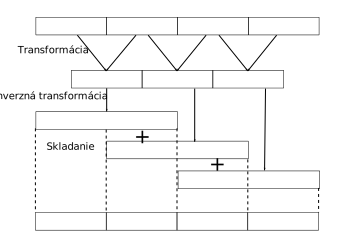
\includegraphics{obrazky/informatika/audio/lapped_transform}
    \caption{Schéma prekladanej transformácie}
    \label{fig:lapped_transform}
\end{figure}

Vzorec Modifikovanej diskrétnej kosínovej transformácie je
\begin{equation}
  X_k = \sum_{i=0}^{2*N-1} x_i 
            \cos(\pi /N (i + 1/2 + 1/2 N) (k + 1/2)),
            \quad k \in 0,1,\dots N-1
\end{equation}
A inverzná transformácia je
\begin{equation}
  x_k = \sum_{i=0}^{N-1} X_k 
            \cos (\pi/N (k + 1/2 + 1/2 N) (i + 1/2)),
            \quad k \in 0,1,\dots 2N-1
\end{equation}

Samotná MDCT ešte nerieši problém, ktorý sme načrtli na začiatku.
Síce v rámci jedného dvojbloku je výsledok spojitý,
na rozhraní blokov môžu ale stále vznikať veľké skoky.
Preto je našou snahou eliminovať tieto skoky. Jednoduchým spôsobom ako
zaručiť ich elimináciu je predpokladať, že signál na krajoch dvojbloku
konverguje k nule. Otázkou ostáva, ako to zaručiť. Tu sa ukazuje
výhodná technika takzvaného windowing-u. Umelo znížime váhu krajov
dvojblokov pri sčítaní, niečo ako plynulý prechod od medzi použitými
dvojblokmi. Najjednoduchší postwindowing môžeme vidieť na
nasledujúcom obrázku.
\begin{figure}[htp]
    \centering
    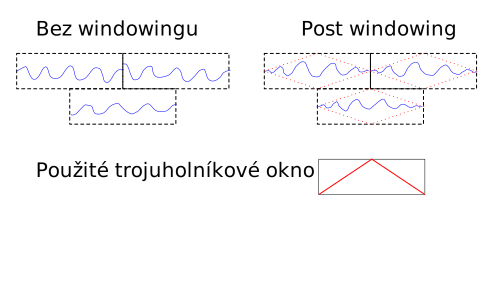
\includegraphics{obrazky/informatika/audio/post_windowing}
    \label{fig:post_windowing}
    \caption{Ukážka funkcie windowingu}
\end{figure}[htp]
\begin{poznamka}
    Pri windowed transformácii sa bežne výsledok násobí konštantou 2.
    Toto je nepísaná dohoda, aby rovnica okna vyzerala krajšie.
    Špeciálne, aby okno dosahovalo maximálnu hodnotu 1.
\end{poznamka}
Samozrejme, ukážkové trojuholníkové okno nie je optimálne.
V reálnych aplikáchiach sa používajú sofistikovanejšie okná.
Navyše, signál so windowuje nielen po transformácii ale aj pred. Toto
možno pôsobí divne, ale spomeňme si, že najväčší skok daného
(dvoj)bloku je práve medzi začiatkom a koncom. Tento skok za pomoci
Gibbsovho fenoménu prináša zbytočné zvonenie a tak zamedzuje dobrej
kompresii.

V praxi najbežnejším pre- aj post- oknom je takzvané sínusové okno
(rovnica \ref{eq:sine_window}),

\begin{equation}
    W_i = \sin(\pi/n (i + 1/2)),\quad  i\in 0,1,\dots n-1
    \label{eq:sine_window}
\end{equation}

ktorého priebeh pre $n=128$ je znázornený na obrázku
\ref{fig:sine_window}. Sínusové okno sa používa napríklad v MP3 a AAC
formátoch.

\begin{figure}[htp]
    \centering
    \includegraphics{obrazky/informatika/audio/sine_window}
    \caption{Sínusové okno pre $n=128$}
    \label{fig:sine_window}
\end{figure}

Aby sme demonštrovali význam modifikovanej transformácie, pripravili
sme porovnanie reakciu DCT a MDCT na zmenu koeficientov (či už
filtrovaním alebo kvantizovaním).
Na obrázku \ref{fig:dct_vs_mdct} je zobrazené porovnanie diskrétnej
kosínovej transformácie a jej modifikovanej verzie so sínusovým oknom.
Pôvodný signál sme transformovali, aplikovali náhodný šum (simulovanie
kvantizácie) a transformovali inverzne. Obrázok je výrez celého
signálu ukazujúci hranicu medzi dvoma po sebe idúcimi blokmi.
\begin{figure}[htp]
    \centering
    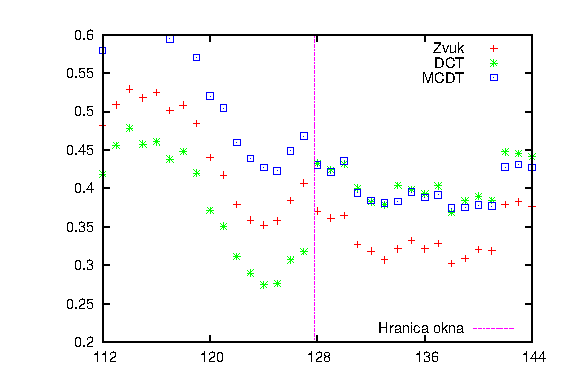
\includegraphics{obrazky/informatika/audio/dct_vs_mdct}
    \caption{Porovnanie DCT a MDCT so sínusovým oknom}
    \label{fig:dct_vs_mdct}
\end{figure}

\subsubsection{Psychoakustický model}
Ľudia nevnímajú zvuk rovnako na všetkých frekvenciách. Toto je dané
stavbou ľudského ucha a spracovaním signálov v mozgu. Psychoakustika
sa zaoberá týmto vnímaním a vypracovalo sa veľké množstvo štúdii
venujúcich sa tejto problematike. My do tejto tematiky načrieme iba jemne
a vyberieme najdôležitejšie závery, ktoré sa priamo týkajú
kompresie zvuku. Časti signálu, ktoré človek nemôže počuť, totiž vôbec
nemusíme uchovávať - je to zbytočné. Pri kompresii je teda snahou čo
najviac oddeliť potrebný signál od nepotrebného a potrebný kvantizovať
menšími koeficientami.

Základným kameňom psychoakustického modelu sú takzvané "equi-loudness"
krivky, zobrazujúce ako silno vníma ľudské ucho zvuk. Vo všeobecnosti,
2 zvuky o rôznej frekvencii a rovnakej intenzite človek nevníma rovnako hlasno.
Zavádza sa preto jednotka "són", ktorá reprezentuje počuteľnú
intenzitu. 1 són je definovaný ako vnímaná hlasitosť tón s frekvenciou
1kHz a intenzitou 40dB. Na obrázku \ref{fig:equi_loudness} je
znázornená prerušovanou čiarou hladina počuteľnosti. Akýkoľvek zvuk
tichší ako daná hladina je pre človeka nepočuteľný a preto ho netreba
uchovávať. Je jasne viditeľné, že človek vníma najlepšie zvuk o
frekvencii 4kHz a nízke či veľmi vysoké frekvencie už vôbec nevníma.

\begin{figure}[htp]
    \centering
    \includegraphics{obrazky/informatika/audio/equi_loudness}
    \caption{Vnímanie zvuku ľudským uchom}
    \label{fig:equi_loudness}
\end{figure}

Okrem základnej hladiny počuteľnosti sa počuteľnosť mení aj takzvaným
maskovaním.
Maskovanie nastáva, keď jeden zvuk ostane nepočuteľný kvôli druhému. V
psychoakustike rozlišujeme dva rôzne typy maskovanie - časové a
simultánne.

Simultánne maskovanie nastáva ako súzvuk dvoch rôznych zvukov/tónov v tom
istom čase. Príkladom môže byť rozhovor vedený pri rušnej ceste.
Zakaždým keď prechádza auto, rozhovor menej počuť. Maskovanie sa
pritom prejavuje tým výraznejšie, čím sú dané 2 tóny bližšie k sebe,
jednak vo frekvencii a jednak v čase. Ukážku simultánneho maskovania
môžeme vidieť na obrázku \ref{fig:simultaneous_masking}. Podľa
obrázka, tón o frekvencii 1kHz môže maskovať dokonca až 1 oktávu nadol
a 2 oktávy nahor. Taktiež vidno, že maskovanie je spravidla väčšie
smerom k vyšším frekvenciám.

\begin{figure}[htp]
    \centering
    \includegraphics{obrazky/informatika/audio/simultaneous_masking}
    \caption{Simultánne maskovanie tónom frekvencie 1kHz}
    \label{fig:Simultaneous_masking}
\end{figure}

Temporálne alebo časové maskovanie naopak maskuje tóny ktoré sa rýchlo
striedajú za sebou. Za (ale aj pred) hlasným tónom chvíľu nepočuť
tichší tón, hoci môže znieť presne od okamihu skončenia hlasného tónu.
Spätná maskovanie (maskovanie, kedy maskér nasleduje až po maskovanom
tóne) je pomerne krátke, efektívne trvá do 2-3 milisekúnd.
Naopak, dopredné maskovanie podľa obrázka \ref{fig:temporal_masking}
môže trvať aj cez 15ms.

\begin{figure}[htp]
    \centering
    \includegraphics{obrazky/informatika/audio/temporal_masking}
    \caption{Ukážka časového maskovania}
    \label{fig:temporal_masking}
\end{figure}

Miesto potrebné na uloženie údajov sa dá redukovať ešte ďalej.
Typicky, stereofónny zvuk má podobný ľavý a pravý kanál. Toto
pozorovanie sa dá ľahko využiť - ak namiesto $L,R$ použijeme
$\frac{L+R}{2}, \frac{L-R}{2}$, dostaneme prvú zvukovú stopu, ktorá je
akoby monofónna verzia a navyše dostaneme informáciu ako mono premeniť
na stereo. Táto druhá stopa je typicky menej náročná na dátový tok.
Spracovanie zvuku týmto spôsobom sa nazýva Joint Stereo.
Stále sa ale dá pokračovať v tomto smere. Jednou z vlastností ľudského
vnímania zvuku je neschopnosť rozlíšiť smer z ktorého prichádzajú
veľmi vysoké tóny. Preto tóny o vysokých frekvenciách (a podobnej
intenzite v ľavom a pravom kanále) môže byť uložené mono, nakoľko je
to pre ucho nerozpoznateľné.

\subsubsection{Kompresia}

Na obrázku \ref{fig:mp3_flow_diagram} je znázornený postupný priebeh
kompresie obľúbeného zvukového formátu mp3, na ktorom si demonštrujeme
kompresiu zvuku. Na vstupe je zvuk v digitálnej podobe nasnímaný po
snímkoch. Daný zvuk sa najskôr rozdelí na 32 frekvenčných pásiem,
ktoré sa čiastočne prekrývajú. Rozdelenie do pásiem umožňuje lepšiu
aplikáciu MDCT. Vstupný zvuk sa zároveň spracuje pomocou štandardnej
Fourierovej transformácie, ktorá poslúži psychoakustickému modelu ako
podklad na určenie kvantizácie. Výstup z psychoakustického modelu sa
priamo aplikuje na MDCT ako veľkosť použitého okna. Pre dynamické
zvuky sa používa kratšie okno ako napríklad pre dlhé tiché pasáže.
Po windowingu je výstup MDCT nasmerovaný ho hlavnej časti kodeku.
Tou je kvantizácia, kde sa kodek snaží nájsť optimálnu sadu
kvantizačných koeficientov, aby jednak vyhovel požadovanému bitovému
toku a jednak zachoval čo najnižšie skreslenie signálu. Výstup po
kvantizovaní potom putuje na klasické kódovanie entropie, pomocou
Huffmanovho kódovania.

\begin{figure}[htp]
    \centering
    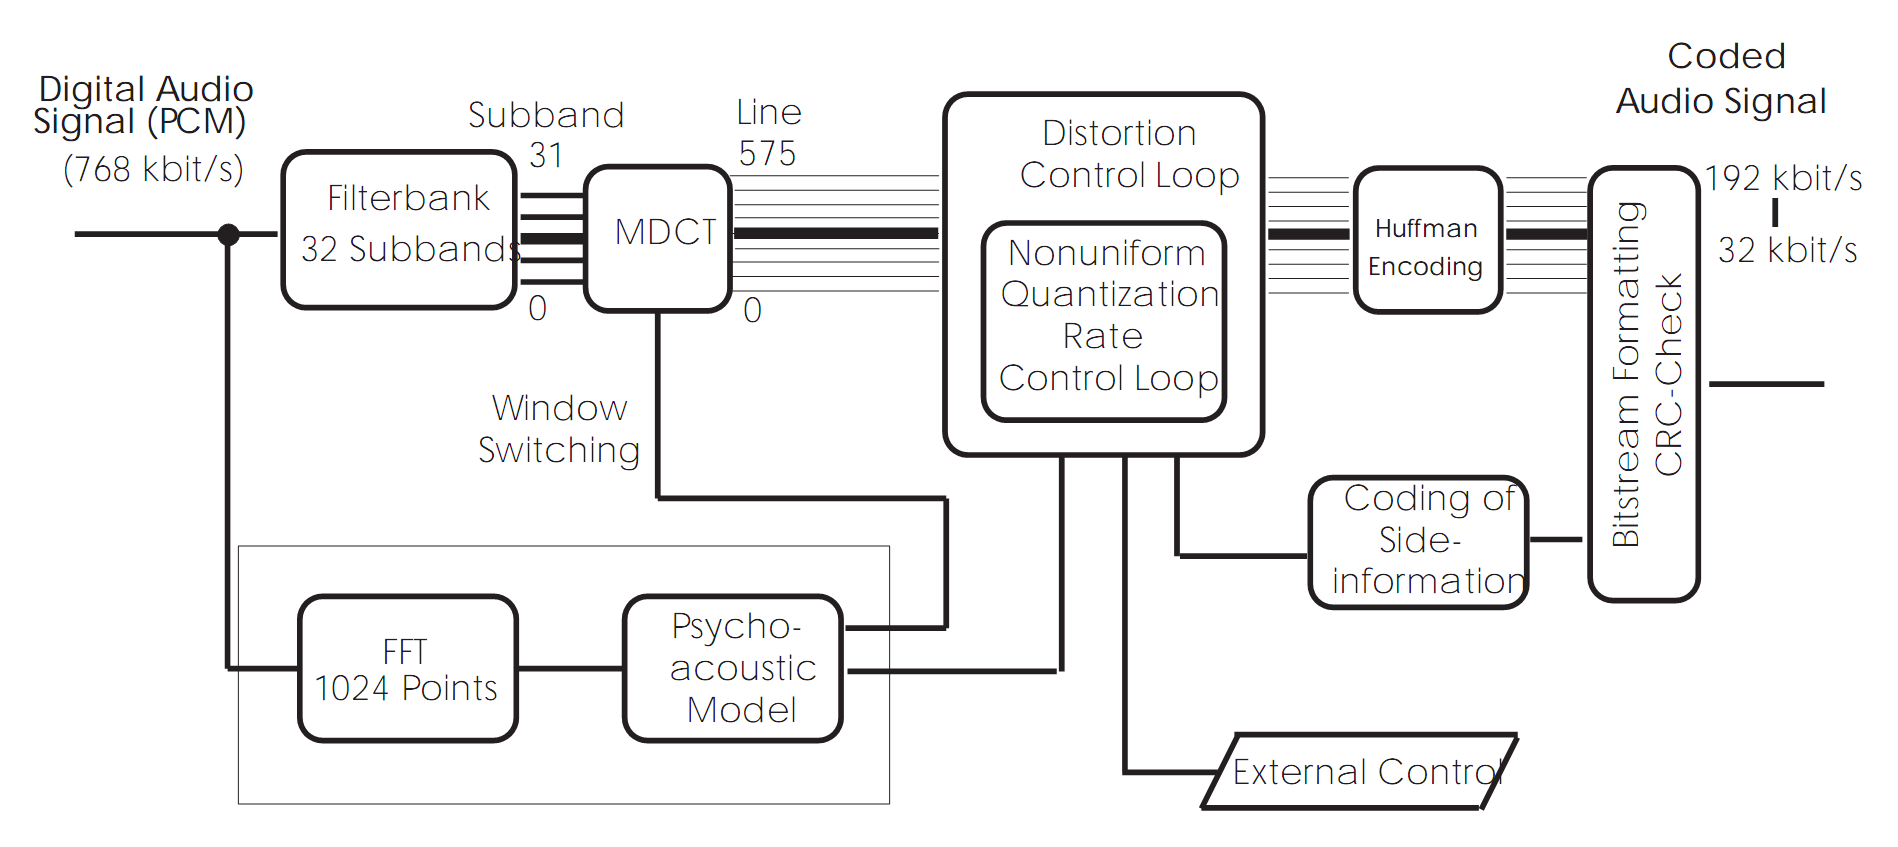
\includegraphics{obrazky/informatika/audio/mp3_flow_diagram}
    \caption{Blokový diagram priebehu kompresie vo formáte mp3}
    \label{fig:mp3_flow_diagram}
\end{figure}

\todo{lit:mp3aac}
